\documentclass{article}
\usepackage[utf8]{inputenc}
\usepackage[serbian]{babel}

\usepackage{graphicx}
\graphicspath{ {./images/} }

\title{Prepoznavanje pokreta ruku}
\author{Jovana Đurović \and Danilo Matić}
\date{Septembar 2022.}

\begin{document}

\maketitle

\newpage

\section{Uvod}

Ljudska aktivnost i prepoznavanje gestova, kao jedni od veoma bitnih komponenti veoma širokog i brzo rastućeg domena ambijentalne inteligencije, mogu biti predmet velikog broja istraživanja, baš zbog njihovog širokog spektra primene. U ovom radu ćemo se fokusirati na pokrete/gestove ruke, čiji jedan kontekst primene može biti ambijentalno praćenje u pametnim kućama, kao i upravljanje raznim pametnim uređajima(telefoni, satovi, dronovi...). Kombinovali smo dve tehnike deep learning-a, konvolutivne neuronske mreže (CNN) i rekurentne neuronske mreže (RNN), kako bismo prepoznali automatizovani pokret rukom koristeći podatke o skeletu ruke (u nastavku skeleton podaci).


\subsection{Naučni doprinosi drugih istraživača na temu Prepoznavanje pokreta rukom zasnovano na skeleton podacima}
Do sada, u naučnom svetu, mnogo više interesovanja je bilo za prepoznavanje pokreta celog tela, umesto prepoznavanje pokreta rukom, ali u nastavku ćemo predstaviti istraživače koji su svojim radovima obezbedili veliki doprinos.

Do sada, u naučnom svetu, mnogo više interesovanja je bilo za prepoznavanje pokreta celog tela, umesto prepoznavanja pokreta rukom, ali porast interesovanja za ovu temu raste eksponencijalno sa razvojem tehnologije i sa sve većom prisutnosti ambijentalne inteligencije u našim svakodnevnim životima. U nastavku ćemo pomenuti neke od značajnih radova na ovu temu.

B. Ioenescu je 2005. godine predložio da se koristi tehnika dinamičkog prepoznavanja pokreta rukom, bazirana na 2D skeleton reprezentaciji ruke. Za svaki pokret, bila bi generisana slika pomoću superpozicije skeleta u svakom držanju, što je smatrano dinamičkim potpisom tog gesta. Faza prepoznavanja se sastojala od računanja Baddeley-eve udaljenosti ovog potpisa u odnosu na celi skupa pokreta.

Uz razvoj tehnologije, i ideje su postale naprednije.

Wang i Chan su 2014. koristili mapu dubine i skeleton dobijeni pomoću Kinect uređaja. Kinect uređaji uglavnom sadrže RGB kamere, infracrvene projektore i detektore koji mapiraju dubinu kroz strukturirano svetlo ili proračune vremena leta, što se zauzvrat može koristiti za prepoznavanje pokreta u realnom vremenu i detekciju skeleta tela, između ostalih mogućnosti. Oblici ruke(dubina) i odgovarajuće teksture su predstavljeni kao superpikseli. Na osnovu ovakve reprezentacije podataka, predlažu da se pomoću EMD (Earth Mover's) udaljenosti izmeri neslaganje između različitih pokreta rukom.

De Smedt je 2016. je razmatrao skelet ruke korišćenjem Intel RealSense kamere, koja nudi mogućnost predstavljanja skeleta ruke pomoću koordinata 22 zgloba šake u 3D-u. Da bi predstavili pokret ruke, autori su predložili da se prati evolucija pokreta ruke kroz vreme na osnovu pokreta zglobova, kao i translacionih i rotacionih pokreta ruke. Pomoću ove kamere generisan je i naš skup podataka.



\section{Implementacjia}

\subsection{Ulazni podaci}
DHG 14/28 (DataSet HandGesture 14/28)\newline

DHG 14/28 sadrži sekvence od 14 različitih pokreta ruke, koji su izvođeni na 2 načina:\newline
1.pomoću jednog prsta\newline
2.korišćenjem cele šake\newline
Svaki pokret je izveden 5 puta od strane 20 učesnika, na dva različita načina i to rezultira 14*5*20*2 = 2800 sekvenci, po čemu je i ovaj skup dobio ime. Svi učesnici su desnoruki. Sekvence su označene prema njihovom pokretu, broju korišćenih prstiju, izvođacu i uspešnosti.\newline
Svaki frejm sekvence sadrži:\newline
1. sliku dubine\newline
2. koordinate 22 zgloba u 2D-u i 3D-u čineći skelet pune ruke.\newline
Kao što je već pomenuto, za prikupljanje skupa podataka koristi se Intel RealSense kamera kratkog dometa. Dubinske slike i skeleti ruku su snimljeni u 30fps, sa rezolucijom dubinske slike 640x480. Dužina uzorka gestova ruke se kreće 20-50 frame-ova.\break

S obzirom na performanse računara koje koritimo i na složenost same implementacije ukoliko se koriste i dubinski podaci ruke zajedno sa skeleton podacima, kao i složenosti samog skupa podataka, naš model obučavamo samo na skeleton podacima.\break

Fajlovi skupa podataka imaju sledeću strukturu:

\begin{figure}[ht]
\centering
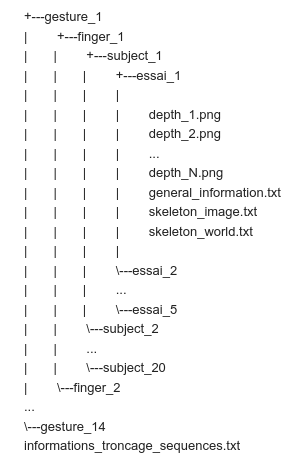
\includegraphics[scale=0.4]{datasetOpis.png}
\caption{Struktura dataseta}
\end{figure}

\newpage



Za sekvencu veličine N:
\begin{itemize}
    \item depth\_n.png sadrži sliku dubine(broj bitova koji se koriste za predstavljanje svakog piksela na slici) n-tog frejma sekvence
    \item general\_information.txt sadrži matricu veličine Nx5. Format je sledeći: Vremenski okvir od 10-7 sekundi i region ruke od interesa u tom okviru predstavljeni slikom dubine (x,y,širina,visina)
    \item skeleton\_image.txt sadrži matricu veličine Nx44. Svaka linija sadrži 2D koordinate zglobova ruke u prostoru slike dubine. Format je sledeći: x1y1 - x2y2 - ... - x22y22.
    \item skeleton\_world.txt sadrži matricu veličine Nx66. Svaka linija sadrži 3D koordinate zglobova ruke u svetu. Format je sledeći: x1y1z1 - x2y2z2 - ...- x22y22z22.
\end{itemize}



informations\_troncage\_sequences.txt sadrži matricu veličine 2800x6. Svaka linija ima sledeći format: \#gest - \#prst - \#izvodilac - \#pokusaj pokreta i sve dodatne- \# frejm kada pocinje pokret - \# frejm zavrsetka izvođenja pokreta.

\subsubsection{Učitavanje podataka}
Pre kreiranja modela neophodno je razumeti i pripremiti podatke koji se
koriste. Skup podataka koji se korsiti u ovom projektu sadrži odgovarajuće
fajlove koji predstavljaju skeleton koordinate svakog pokreta.

Fajlove skeletonimage.txt je potrebno dodatno pripremiti kako bi mogli da se
koriste za treniranje i testiranje modela, što je omogućeno njihovim skaliranjem tako da bi se postigla jednakost za sve skeleton podatke svakog pokreta.

\subsubsection{Priprema podataka za obučavanje}
Podatke delimo na podatke za treniranje i za testiranje u odnosu 70:30.
Imena pokreta, koja su označena numerički od 1 do 14, pretvaramo u binarnu matricu koja predstavlja ulaz.
Same skupove za trening i testiranje preoblikujemo tako tako da budu oblika (veličina skupa, 1, broj skeleton podataka po pokretu, veličina jednog skeleton podatka jednog pokreta) 
ili (veličina skupa, kanal, broj skeleton podataka po pokretu, veličina jednog skeleton podatka jednog pokreta,1) ukoliko kanal nije na početku.

\newpage

\subsection{Kreiranje neuronske mreže}

Glavni deo projekta predstavlja pravljenje i obučavanje neuronskih mreža.
Na osnovu podataka treba izabrati koju mrežu je pogodno koristiti. Podatke
koji predstavljaju pokrete posmatramo kao matrice koordinata skeletona ruke.
Pošto obrada dinamičkih prepoznavanja pokreta zavisi od uređenog niza
koordinata skeletona ruke, koristimo RNN na izlasku iz CNN-a koji bolje radi sa sekvencama podataka u odnosu na CNN.
\subsubsection{Parametri}

Struktura konvolutivne neuronske mreže se sastoji iz 6 konvolutivnih slojeva veličine 3*3 od kojih svaki koristi "relu" aktivacionu funkciju. Između svakog drugog sloja se nalazi agregacioni sloj sa funkcijom maksimuma.
Na izlaz iz konvolutivnog dela mreže je primenjen dropout sloj radi sprečavanja
preprilagođavanja, a zatim jedan flatten sloj za poravnavanje.
Sledeći sloj je rekurentna neuronska mreža koja se sastoji od jednog "Long Short Term Memory" (LSTM) sloja.
Izlaz iz rekurentnog dela mreže predstavlja ulaz u potpuno povezani deo koji se
sastoji od tri usko povezana sloja. Prva dva koriste "relu" aktivacionu funkciju dok poslednji sloj ima softmax aktivacionu funkciju. Između svakog sloja se nalazi jedan dropout sloj. 

Kao optimizator je korišćen ”adam” funkcija. Kategorička unakrsna entropija je korišćena kao funkcija greške, dok nam metriku za kvalitet modela predstavlja tačnost. Model je treniran na 100 epoha. 


\begin{figure}[ht]
\hbox{\hspace{-3em} 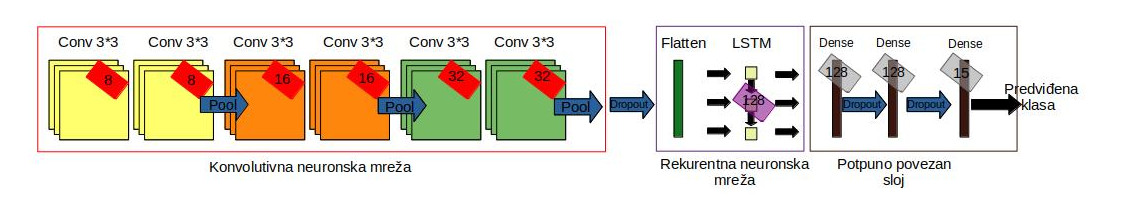
\includegraphics[scale=0.5]{model.jpg}}
\caption{Struktura modela}
\end{figure}


\newpage

\section{Rezultati}

Kvalitet modela procenjujemo na osnovu test skupa. To je skup koji nismo koristili za obučavanje modela. Zbog toga je merodavna ta ocena.
Dobijeni CNN + RNN model pokazuje tačnost oko 94\%. Mere tačnosti i greške se računaju tokom svake epohe obučavanja modela. Na slici 2. su prikazani grafici Mere greške i tačnosti.

\begin{figure}[h]
\centering
\hbox{\hspace{-3em} 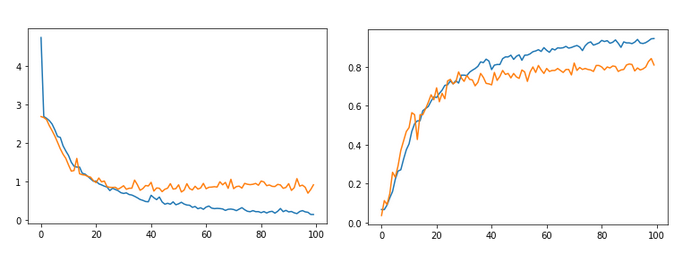
\includegraphics[scale=0.6]{grafik}}
\caption{Mere greške i tačnosti kroz epohe}
\end{figure}

Za analizu kvaliteta modela nam je korisna i matrica konfuzije. Matrica konfuzije je matrica u kojoj njen element $x_{ij}$ predstavlja broj istanci klase $i$ koje je dati model klasifikovao kao klasu $j$. Na dijagonali se nalaze ispravno klasifikovane istance.

\begin{figure}[h]
\centering
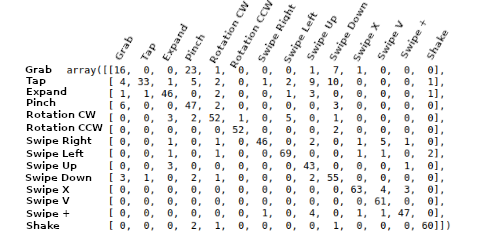
\includegraphics[scale=0.65]{matricaKonfuzije.png}
\caption{Matrica konfuzije}
\end{figure}

\newpage

Analizom dobijene matrice konfuzije možemo da uočimo da model dobro klasifikuje različite pokrete. Primećujemo da model najčešće pogrešno klasifikuje "Pinč" pokret umesto "Grab" pokreta (polje $x_{03}$).
\newline

Dobijene rezultate ćemo uporediti sa rezultatima modela koji su pravili H.Mahmud, M. M. Morshed i Md. K. Hasan u novembru 2021. godine.
\newline

Njihov rad se razlikuje od radova ostalih istraživaca po tome što su primetili da neobrađene slike dubine poseduju nizak kontrast u predelima šake. Ne ističu važne detalje, kao što su orijentacija prsta, preklapanje između prsta i dlana, ili preklapanje između više prstiju. Oni predlažu kvantovanje vrednosti dubine u nekoliko diskretnih regiona, da bi se stvorio veći kontrast između nekoliko ključnih delova ruke. Takođe, naglasili su da su modeli ostalih istraživača bili pre-parametrizovani. Dodatno, predlažu nekoliko načina za rešavanje problema visoke varijanse u postojecim CRNN arhitekturama. Oni su svoj model obučavali na dva skupa podataka: SHREC-17 i DHG-14/28, pa je zato pogodno za upoređivanje rezultata, iako su ovi istraživaci koristili i podatke o dubini, kao i podatke o 2D skeletu. Fokusirali su se na samu ulaznu reprezentaciju podataka, kao i na specifikacije hardvera kako bi obezbedili što bolje rezultate.
\newline


Njihov pristup je doveo do tačnosti od 90.21\% za predviđanje 14 pokreta i 88.4\% za predviđanje 28 pokreta na skupu DHG-14/28, čime su nadmašili dosadašnje najbolje postignute rezultate u ovoj oblasti, koje su postigli K.Lai i S. N. Yanushkevich 2018. godine(85,46\% i 74,19\% na 14 i 28 gestova).
\newline

Iako su rezultati izvaredni, njihov model se susreće sa istim problemom na koji naš model nailazi, a to je razlikovanje pokreta Grab i Pinch.



\newpage

\section{Zaključak}

U ovom radu je predstavljen jedan od pristupa pogodnih za prepoznavanje pokreta ruke. Ovaj pristup korsti konvulutivne i rekurente mreže. Model je obučavan na skupu podataka DHG-14/28. Važno je naglasiti da pri obučavanju modela nisu korišćeni podaci o dubini slika, već samo skeleton podaci, što značajno utiče na samu implementaciju i tačnost modela, kao i upotrebu modela u realnom svetu.

\newpage

\begin{thebibliography}{6}

    \bibitem{DhgSkeleton}
    B. Ionescu, D. Coquin, P. Lambert, V. Buzuloi, Dynamic hand gesture recognition using the skeleton of the hand, EURASIP J. Appl. Signal Process. 13 (2005)2101–2109, doi:10.1155/ASP.2005.2101.


	\bibitem{dhgColor_depth}
	C. Wang, S.C. Chan, A new hand gesture recognition algorithm based on joint color-depth superpixel earth mover’s distance, 4th International Workshop on Cognitive Information Processing (CIP), 2014, doi:10.1109/CIP.2014.6844497
	
	\bibitem{DHGSkeletonIEEE}
	 Q. De Smedt, H. Wannous, J.P. Vandeborre, Skeleton-based dynamic hand gesture recognition, in: The IEEE Conference on Computer Vision and PatternRecognition Workshops (CVPRW), 2016, pp. 1206–1214, doi:10.1109/CVPRW.2016.153.

	\bibitem{CNNRNN}
	J. C. Núñez, R. Cabido, J.J. Pantrigo, A. S. Montemayor, J. F. Vélez,Convolutional Neural Networks and Long Short-Term Memory for skeleton-based human activity and hand gesture recognition,Pattern Recognition, ISSN 0031-3203

    \bibitem{Svetlana}
    K. Lai and S. N. Yanushkevich, "CNN+RNN Depth and Skeleton based Dynamic Hand Gesture Recognition," 2018 24th International Conference on Pattern Recognition (ICPR), 2018, pp. 3451-3456, doi: 10.1109/ICPR.2018.8545718.


\end{thebibliography}


\end{document}